%%%%%%%%%%%%%%%%%%%%%%% file template.tex %%%%%%%%%%%%%%%%%%%%%%%%%
%
% This is a general template file for the LaTeX package SVJour3
% for Springer journals.          Springer Heidelberg 2010/09/16
%
% Copy it to a new file with a new name and use it as the basis
% for your article. Delete % signs as needed.
%
% This template includes a few options for different layouts and
% content for various journals. Please consult a previous issue of
% your journal as needed.
%
%%%%%%%%%%%%%%%%%%%%%%%%%%%%%%%%%%%%%%%%%%%%%%%%%%%%%%%%%%%%%%%%%%%
%
% First comes an example EPS file -- just ignore it and
% proceed on the \documentclass line
% your LaTeX will extract the file if required
\begin{filecontents*}{example.eps}
%!PS-Adobe-3.0 EPSF-3.0
%%BoundingBox: 19 19 221 221
%%CreationDate: Mon Sep 29 1997
%%Creator: programmed by hand (JK)
%%EndComments
gsave
newpath
  20 20 moveto
  20 220 lineto
  220 220 lineto
  220 20 lineto
closepath
2 setlinewidth
gsave
  .4 setgray fill
grestore
stroke
grestore
\end{filecontents*}
%
\RequirePackage{fix-cm}
%
%\documentclass{svjour3}                     % onecolumn (standard format)
%\documentclass[smallcondensed]{svjour3}     % onecolumn (ditto)
\documentclass[smallextended]{svjour3}       % onecolumn (second format)
%\documentclass[twocolumn]{svjour3}          % twocolumn
%
\smartqed  % flush right qed marks, e.g. at end of proof
%
\usepackage{graphicx}
%
% \usepackage{mathptmx}      % use Times fonts if available on your TeX system
%
% insert here the call for the packages your document requires
%\usepackage{latexsym}
% etc.
\usepackage[T1]{fontenc}
\usepackage[utf8]{inputenc}
\usepackage{upquote,textcomp}
\usepackage{soul} % used by \hl
\usepackage{hyperref}
\usepackage[left]{lineno} % used by linenumbers
%\usepackage{nameref,hyperref}
%\usepackage{cite}
%\usepackage{textcomp,marvosym}
%\usepackage{fixltx2e}
%\usepackage{changepage} % used by adjustwidth
\usepackage{apacite}
%
% please place your own definitions here and don't use \def but
% \newcommand{}{}
%
%\newcommand{\slnote}[1]{{\hl{\small SL: #1}}\,}
\newcommand{\jknote}[1]{{\hl{\small JD: #1}}\,}
%\newcommand{\alka}[1]{{\hl{\small Alko: #1}}\,}
%\providecommand{\url}[1]{\texttt{#1}}
\newcommand{\code}[1]{\texttt{#1}}
\newcommand{\fig}[1]{Fig.~\ref{#1}}


\setcounter{errorcontextlines}{999}
% Insert the name of "your journal" with
% \journalname{myjournal}
%
\journalname{Behavior Research Methods}

\begin{document}

\title{PyMICE -- a Python library for analysis of IntelliCage data
%PyMICE -- facilitating reproducible research with IntelliCage system
%\thanks{Grants or other notes
%about the article that should go on the front page should be
%placed here. General acknowledgments should be placed at the end of the article.}
}
%\subtitle{Do you have a subtitle?\\ If so, write it here}

%\titlerunning{Short form of title}        % if too long for running head

\author{Jakub M. Dzik \and
        Alicja Puścian \and
        Zofia Mijakowska \and
        Kasia Radwanska \and
        Szymon Łęski
}

%\authorrunning{Short form of author list} % if too long for running head

\institute{J. M. Dzik \and A. Puścian \and S. Łęski \at
              Department of Neurophysiology, Nencki Institute of Experimental Biology of Polish Academy of Sciences, Warsaw, Poland \\
%              Tel.: +123-45-678910\\
%              Fax: +123-45-678910\\
%              \email{fauthor@example.com}           %  \\
%             \emph{Present address:} of F. Author  %  if needed
           \and
           Z. Mijakowska \and K. Radwanska \at
              Department of Molecular and Cellular Neurobiology, Nencki Institute of Experimental Biology of Polish Academy of Sciences, Warsaw, Poland
           \and
           S. Łęski \at \email{s.leski@nencki.gov.pl}
}

\date{Received: date / Accepted: date}
% The correct dates will be entered by the editor


\maketitle

\linenumbers

\begin{abstract}
IntelliCage is an automated system for recording the behavior of a group of mice 
housed together. It produces rich, detailed behavioral data calling for new 
methods and software for their analysis. Here we present PyMICE -- a free and open source
library for analysis of IntelliCage data in Python programming language. 
We describe the design and demonstrate the use of the library through 
a series of examples.  PyMICE provides easy and intuitive 
access to IntelliCage data, and thus facilitates the possibility of using 
numerous other Python scientific libraries to form a complete data analysis workflow.

%Insert your abstract here. Include keywords, PACS and mathematical
%subject classification numbers as needed.
\keywords{Python \and library \and mice \and behavior \and analysis \and IntelliCage}
% \PACS{PACS code1 \and PACS code2 \and more}
% \subclass{MSC code1 \and MSC code2 \and more}
\end{abstract}

\section{Introduction}
\label{intro}

In recent years, a number of automated environments for behavioral testing
have been developed, based on
RFID~\cite{Dellomo:1998ts,Galsworthy:2005br,Daan:2011wl,EcoHABfullyauto:2015tk}
or video tracking of
animals~\cite{deChaumont:2012du,Weissbrod:2013bc,Shemesh:2013be,PerezEscudero:2014ed}.
Such automated systems have many advantages compared to the traditional behavioral tests,
such as the
reduction of the animal stress caused by isolation and
handling~\cite{Heinrichs:2006dk,Sorge:2014fb},
the possibility of studying social interactions in group-housed
animals~\cite{Kiryk:2011tk},
the possibility of long-term studies,
and easier standardization of protocols in turn leading to better
reproducibility of results between
laboratories~\cite{Crabbe:1999vf,Chesler:2002wo,Krackow:2010ck,Codita:2012jv,Morrison:2014cn,Vannoni:2014jt}.

The system we are particularly interested in is the IntelliCage
system~\cite{intelliCagePlusManual2011,Kiryk:2011tk,Radwanska:2012fd,Puscian:2014cu,Mijakowska:2015io}
(see \fig{intellicageSystem}), which is increasingly popular in behavioral research on
rodents~\cite{IntelliCageReferenceList}.

The system outputs a large amount of data
describing the behavior of the mice in the conditioning corners of the cage.
A typical experiment yields
10,000--100,000 visits recorded during several weeks or months.
Such large data call for development of data analysis methods
and software. One way to address the need of data analysis is to develop a
dedicated application, preferably with a graphical user interface (GUI),
which would allow researchers to inspect the data and extract relevant quantities
interactively. In fact, such an application, called Analyzer, is
provided with the IntelliCage system. While an
interactive GUI-based program for data analysis may be
useful, it does have certain limitations. In the context of scientific research,
perhaps the most severe limitation is poor reproducibility of the analysis,
unless strict measures are taken to record
every single action of the user. Moreover, there is usually no automated
way to perform exactly the same analysis on a different dataset,
and repeating the analysis manually is very time-consuming
and highly error-prone. Another inconvenience of ready-made programs is
that they are typically limited to a predefined set of analysis methods,
and not easily extendable.

Custom data analysis programs (e.g., scripts) fall at the opposite end of the
spectrum than GUI programs. First, the most obvious advantage of such
programs is the essentially unlimited possibility of implementing specialized
analysis methods and applying them much better (in terms of calculation speed,
precision and robustness) than a human.

Second, a noninteractive program (written in any programming language)
running in batch mode is, by
definition~\cite{Hoare69anaxiomatic,Turing1936,Floyd1967Flowcharts,Mccarthy63abasis},
an exhaustive specification of the analysis. In contrast, a plain language
description usually included in a Methods section of a journal article
may be ambiguous or not up-to-date.
The voices calling for providing the data analysis workflows together with
journal publications date at least two decades back~\cite{buckheit1995}:
`an article about computational science in a scientific publication is not
the scholarship itself, it is merely advertising of the scholarship. The
actual scholarship is the complete software development environment and the
complete set of instructions which generated the figures'.

Finally, one of the advantages of using an automated behavioral setup
is the possibility of high-throughput screening
by running the same protocol for a number of mice
cohorts (for example treatment and control groups and/or different strains
of mice~\cite{Puscian:2014cu}). Manual processing of each dataset separately
is both tedious and prone to errors. Batch-processing using a data
analysis script is an obvious remedy, as it allows for repetition of exactly
the same steps of analysis.

The only drawback is that the entry threshold for data analysis using a
programming language is much higher, as significant effort is required to
learn the programming language and necessary technical details (e.g., the data
format).
Our goal here is to lower this threshold by providing an easy and intuitive
way to access the IntelliCage data in the Python programming language~\cite{rossum1995}.

This paper is organized as follows: first, we briefly describe the IntelliCage system.
Next, we introduce PyMICE through a series of examples and provide pointers
to further documentation. We conclude with a short section on technical details and
a discussion.


%Your text comes here. Separate text sections with
\section{IntelliCage system}
\label{sec:1}

\begin{figure*}
  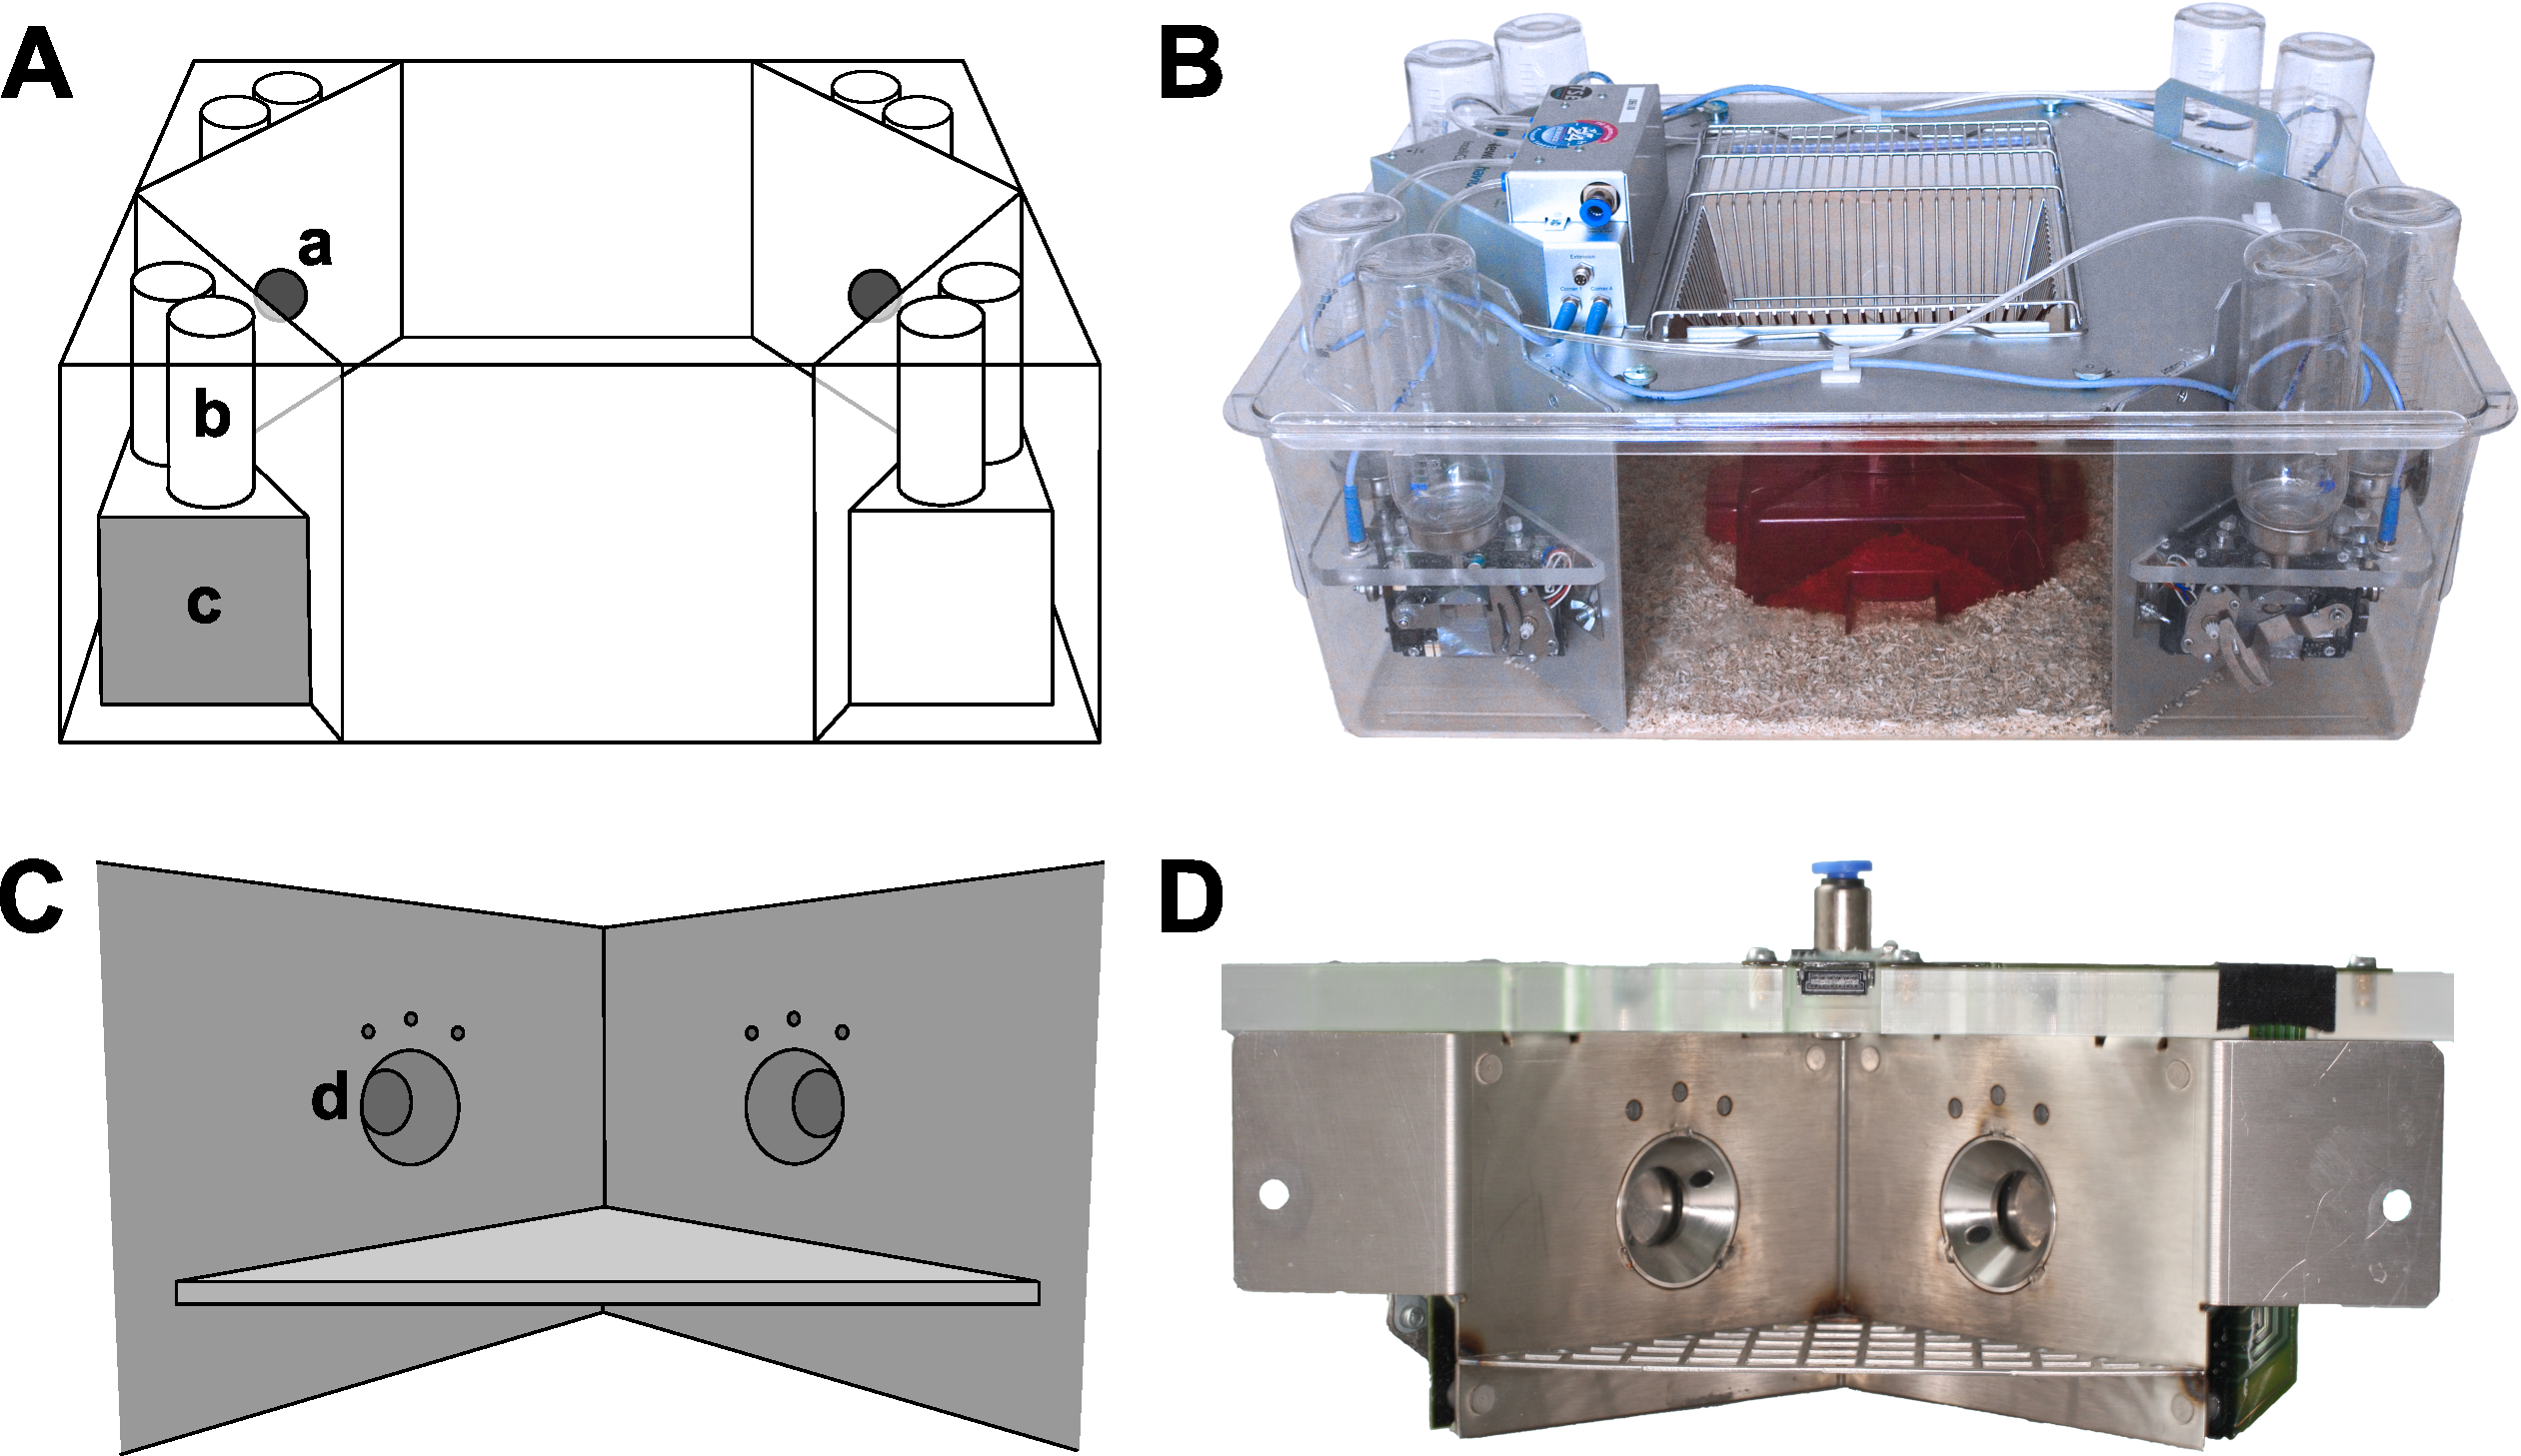
\includegraphics[width=0.75\textwidth]{figures/FigureIC.pdf}
  \caption{
    {\bf IntelliCage system.}
    The system is composed of one or more cages (A,~B).
    Through openings (a) mice can access bottles (b) in a learning chamber (c;~C,~D).
    Access to the bottles is controlled by programmable door in smaller openings in the sides
    of the chamber (d). \emph{Credits:} A, C -- Maria Nowicka, JD; B -- Anna Mirgos, D -- SŁ
  }
  \label{intellicageSystem}
\end{figure*}

IntelliCage (\fig{intellicageSystem}) is an automated, computer-controlled RFID system for
(possibly long-term) monitoring of groups of
mice~\cite{Galsworthy:2005br,Krackow:2010ck,Puscian:2014cu}. The mice are housed in
one or more polycarbonate cages (of size 55 x 37.5 x 20.5 cm;
\fig{intellicageSystem}\textbf{A},~\textbf{B}). A cage can house a group of up to
16 mice. Each mouse is tagged with an RFID transponder.

The key components of the system are learning chambers
(\fig{intellicageSystem}\textbf{c},~\textbf{C},~\textbf{D})
located in the corners of cages
(for brevity, we will refer to the chambers simply as `corners'). Each
corner can be accessed through a circular opening (30 mm in diameter; \fig{intellicageSystem}\textbf{a}),
with an embedded RFID antenna. By design, only one mouse at a time can enter
a corner. Each corner contains two smaller (13 mm in diameter; \fig{intellicageSystem}\textbf{d}) openings,
through which a mouse can access different drinking bottles (\fig{intellicageSystem}\textbf{b}). The access to the
drinking bottles is controlled using programmable doors in
the smaller openings.


A broad range of different experiment protocols can be implemented in the
IntelliCage~\cite{Knapska:2006cz,Kiryk:2011tk,Endo:2011bs,Radwanska:2012fd,Knapska:2013dj,Smutek:2014da,Puscian:2014cu,Vannoni:2014jt}.
The system can be programmed to open the doors on specific conditions, for
instance, if a specific mouse enters the corner or if a specific nosepoke
pattern is performed. Also, an air puff in the back may be delivered to the
mouse as a punishment.

The IntelliCage system records the \textbf{visits} of
each mouse to a particular corner and also tracks the \textbf{nosepokes}
-- which lead to accessing the drinking bottles. When the mouse drinks
from a bottle, the number of \textbf{licks} taken is also recorded.
The events (visits and nosepokes) registered by the system are stored on a
computer as a series of records. Each visit record contains, for example,
the RFID transponder number of a given mouse, the cage and corner,
and the time bounds of the visit. Further,
nosepokes during the visit are also stored, along with
time boundaries and the number of licks recorded, etc.

The system periodically logs the environmental conditions (ambient
illumination and temperature) in every cage connected. It also logs other
relevant events, such as: starts or ends of recording, errors, warnings, and
hardware events (e.g., concerning state of the doors).


\section{PyMICE library}
\label{sec:2}
\input{pymice_overview}

\section{Examples}
\label{sec:3}
In this section we introduce PyMICE through a series of examples illustrating various aspects of the library.\\
In Example 1 we show how to find numbers of visits of a specific mouse in which the first nosepoke was performed to either
the left side or the right side of the corner. 
This can be achieved in PyMICE in just six lines of code. \\
Example 2 is an extension of the Example 1 to analysis
of actual experimental data, obtained with a protocol described in~\cite{Knapska:2013dj}.
In this example we also present a convention for
defining timeline of the experiment. 
\\
In Example 3 we reproduce a plot from an earlier paper~\cite{Puscian:2014cu}.
The plot shows how two cohorts of mice learn the location
of the reward over time (place preference learning). This kind of analysis 
can be performed using Analyzer, the GUI application provided
with IntelliCage; however, using PyMICE we can quickly repeat the analysis for 
new cohorts with minimal effort. \\
Example 4 illustrates how the Python programming language can be used 
to extend the repertoire of data analysis methods.
In this example we show how to extract the information about intervals between visits of different mice to the same corner. 
This kind of information would be very hard (or even impossible) to obtain using Analyzer. 

To improve readability of Examples 2--4 we have omitted some generic code
and focused on PyMICE-specific snippets. Full code of the examples
is provided as online supplementary material at \url{https://github.com/Neuroinflab/PyMICE_SM/tree/examples}.

\input{get_example_data}

In addition to the examples presented here, we have prepared several 
tutorials available online at the PyMICE website~\cite{pymiceWebsite}.
The tutorials are in Jupyter Notebook format~\cite{jupyterOrg} and may be downloaded 
for interactive use. 
The examples and the tutorials are provided as a hands-on introduction to
PyMICE and serve as a starting point for further exploration.
Additionally, online documentation is provided~\cite{pymiceDoc}. PyMICE
objects and their methods are also documented with docstrings available with
Python built in \code{help()} function.
 


\subsection{Example 1: minimal example -- extracting the side of the first nosepokes in 6 lines of code.}
\label{sec:3:1}
\input{example1}

\subsection{Example 2: full analysis example -- side discrimination task.}
\label{sec:3:2}
\input{example2}

\subsection{Example 3: reproducibility -- batch analysis of data.}
\label{sec:3:3}
\input{example3}

\subsection*{Example 4: implementing new behavioral measures -- intervals between visits.}
\label{sec:3:4}
\input{example4} 


\section{Technical details}
\label{sec:4}
We recommend to use the PyMICE library with the Anaconda Python distribution~\cite{anacondaSoftware}.

The library requires \emph{NumPy}~\cite{wald2011,Oliphant:2007ud},
\emph{matplotlib}~\cite{citeulike:2878517}, \emph{dateutil}~\cite{dateutil} and \emph{pytz}~\cite{pytz}
Python packages to be installed in the system.

\begin{samepage}
The library itself is available as a package from the Python Package Index (PyPI)~\cite{pep0301,pypi}
for Python version 3.3, 3.4 and 3.5, as well as 2.7.
It can be installed with either \emph{pip}~\cite{pip}:

\begin{verbatim}
$ pip install PyMICE
\end{verbatim}

or \emph{easy\_install}~\cite{setuptools}:

\begin{verbatim}
$ easy_install PyMICE
\end{verbatim}
\end{samepage}

A bleeding edge version of the library might be also downloaded from
\url{https://github.com/Neuroinflab/PyMICE} GitHub~\cite{github} repository.


\section{Terms of use}
\label{sec:5}
PyMICE library is open-source and is available for free 
under GPL3 license~\cite{gpl}; we ask that this article is cited and resource
identifier~\cite{ozyurt2016} for the library (\emph{RRID:nlx\_158570}) is provided 
in any published research making use of PyMICE.


\section{Discussion}
\label{sec:6}
In this paper we have introduced PyMICE, a software library which allows to access
and analyze data from IntelliCage experiments. 
%
The library has been developed to 
facilitate automated, reproducible, and customizable analysis of large data 
generated by the IntelliCage system. Analyzer, the software bundled with the 
IntelliCage, does not meet these requirements, as it was designed with a 
different purpose in mind~\cite{intelliCagePlusManual2011}:
`The ``Analyzer'' is intended to give an overview of the results [...]
The function of ``Analyzer'' is to provide the user with data merging,
extraction, and filtering tools in order to generate data sets appropriate for
in-depth graphical and statistical analyses.'

One of the features of the IntelliCage system is that very different
experiments are possible, depending on the subject of the research.
Some protocols focus on assessment of subjects' ability of reward
location~\cite{Knapska:2013dj} and behavioral sequence~\cite{Endo:2011bs}
learning. Other protocols are dedicated to measure addiction-related
behavior like subject impulsiveness~\cite{Radwanska:2012fd,Mijakowska:2015io}.
Quite often a new experiment requires a
completely new approach to data analysis. Rather than trying to predict the
specific needs of the prospective users, we decided to provide simple,
intuitive and user-friendly interface for accessing the data. Such interface
allows a scientific programmer to tailor dedicated software focusing on the
essence of the analysis instead of the technical details. To our knowledge,
PyMICE is the only publicly available solution for analysis of IntelliCage 
data in a scripting language.

PyMICE is written in the Python programming language. Our choice of Python 
was directed by the same factors
which made it a popular choice for scientific computing in general. 
Python is free,
open-source, relatively easy to learn, and is supported by a number of
scientific tools and libraries, such as: NumPy and SciPy~\cite{Oliphant:2007ud},
IPython~\cite{Perez:2007wf}, matplotlib,
Pandas~\cite{mckinney-proc-scipy-2010}, etc.
We believe that PyMICE will be a useful addition to that collection.

The number of
IntelliCage-based publications is increasing in recent years~\cite{IntelliCageReferenceList},
but the system is still relatively little known. We believe that one of the factors 
handicapping the popularity of IntelliCage, or similar automated setups, is the lack of a proper 
software ecosystem. We hope that availability of PyMICE will have a stimulating
effect on the adoption of automated behavioral systems. 
While the current (at the time of the publication) version of the library  
only supports the IntelliCage, the library may be generalized to other behavioral systems. 
Data from any system capturing point events (such as
visits to specific locations -- as opposed to e.g. continuous trajectories of the animals) 
could be presented to the user in a similar way as the IntelliCage data. 
Specifically, representing each behavioral event as a Python object
with relevant attributes would allow for intuitive manipulation of data
and for easy extraction of the quantities which are analyzed. 
The PyMICE library is open source~\cite{gpl} and publicly available at
GitHub, the largest open source software platform~\cite{gousios2014}, 
therefore the extensions to other behavioral systems can be contributed by the community. 

A crucial feature of PyMICE is the possibility of creating automated
data analysis workflows. Such workflows are useful, for example, when the same 
protocol is applied to multiple groups of animals -- this is a very common case, 
as most \jknote{of?} experiments will have at least one experimental and one control group. 
A workflow defined in a Python script may be used to perform exactly the same
analysis on every available dataset, which both saves effort and greatly reduces
possibility of mistakes as compared to analyzing each dataset manually.

We also believe that popularization of such workflows would
lead to better research reproducibility. 
Current efforts for reproducible research are mostly focused on improving the
experimental procedures, statistical analysis, and the publishing
policy~\cite{begley2012,begley2013,halsey2015}. However, unclear or ambiguous 
description of data analysis is also given as a factor contributing to 
poor reproducibility of scientific research~\cite{ince2012}. A (non-interactive) 
computer program is a
precise, formal and unambiguous description of the analysis performed.
We hope that PyMICE could become a common platform for implementing
and sharing workflows for analysis of data from the IntelliCage (or similar) system, and
make data analysis using scripts more accesible and more popular.

The paper itself is a proof of the concept of the `really reproducible'
research~\cite{buckheit1995} -- writing it we followed the
literate programming paradigm~\cite{literateProgramming}. Every of the presented
results of analysis was generated by a Python + PyMICE workflow embedded in the
\LaTeX{}~\cite{latex} source code of the document (see the \emph{Statement of reproducibility} below for
details).



\section{Statement of reproducibility\protect\cite{peng2011}}
\label{sec:7}
\input{pymice_reproducibility}

%Text with citations %\cite{RefB} and \cite{RefJ}.
%\subsection{Subsection title}
%\label{sec:2}
%as required. Don't forget to give each section
%and subsection a unique label (see Sect.~\ref{sec:1}).
%\paragraph{Paragraph headings} Use paragraph headings as needed.
%\begin{equation}
%a^2+b^2=c^2
%\end{equation}
%
%% For one-column wide figures use
%\begin{figure}
%% Use the relevant command to insert your figure file.
%% For example, with the graphicx package use
%  \includegraphics{example.eps}
%% figure caption is below the figure
%\caption{Please write your figure caption here}
%\label{fig:1}       % Give a unique label
%\end{figure}
%%
%% For two-column wide figures use
%\begin{figure*}
%% Use the relevant command to insert your figure file.
%% For example, with the graphicx package use
%  \includegraphics[width=0.75\textwidth]{example.eps}
%% figure caption is below the figure
%\caption{Please write your figure caption here}
%\label{fig:2}       % Give a unique label
%\end{figure*}
%%
%% For tables use
%\begin{table}
%% table caption is above the table
%\caption{Please write your table caption here}
%\label{tab:1}       % Give a unique label
%% For LaTeX tables use
%\begin{tabular}{lll}
%\hline\noalign{\smallskip}
%first & second & third  \\
%\noalign{\smallskip}\hline\noalign{\smallskip}
%number & number & number \\
%number & number & number \\
%\noalign{\smallskip}\hline
%\end{tabular}
%\end{table}


\begin{acknowledgements}
JD, KR, and SŁ supported by a Symfonia NCN grant UMO-2013/\allowbreak 08/\allowbreak W/\allowbreak NZ4/\allowbreak 00691. 
AP supported by a grant from Switzerland
through the Swiss Contribution to the enlarged European Union (PSPB-210/2010
to Ewelina Knapska and Hans-Peter Lipp).
KR and ZM supported by an FNP grant POMOST/2011-4/7 to KR.

%If you'd like to thank anyone, place your comments here
%and remove the percent signs.
\end{acknowledgements}

% BibTeX users please use one of
%\bibliographystyle{spbasic}      % basic style, author-year citations
%\bibliographystyle{spmpsci}      % mathematics and physical sciences
%\bibliographystyle{spphys}       % APS-like style for physics
\bibliographystyle{apacite}
\bibliography{pymice,szymonall}%   % name your BibTeX data base


\end{document}
% end of file template.tex

